
\begin{itemize}
    \item Write the results for the RAC building.
    \item Find a system to judge it on.
    \item Mention whether there is or is no ground truth
    \item Manuel planning of route
    \item the results are run on the same script with no of the script between each building. THe only thing changed is the name of the building used.
\end{itemize}
\begin{comment}

\begin{figure}[H]
    \centering
    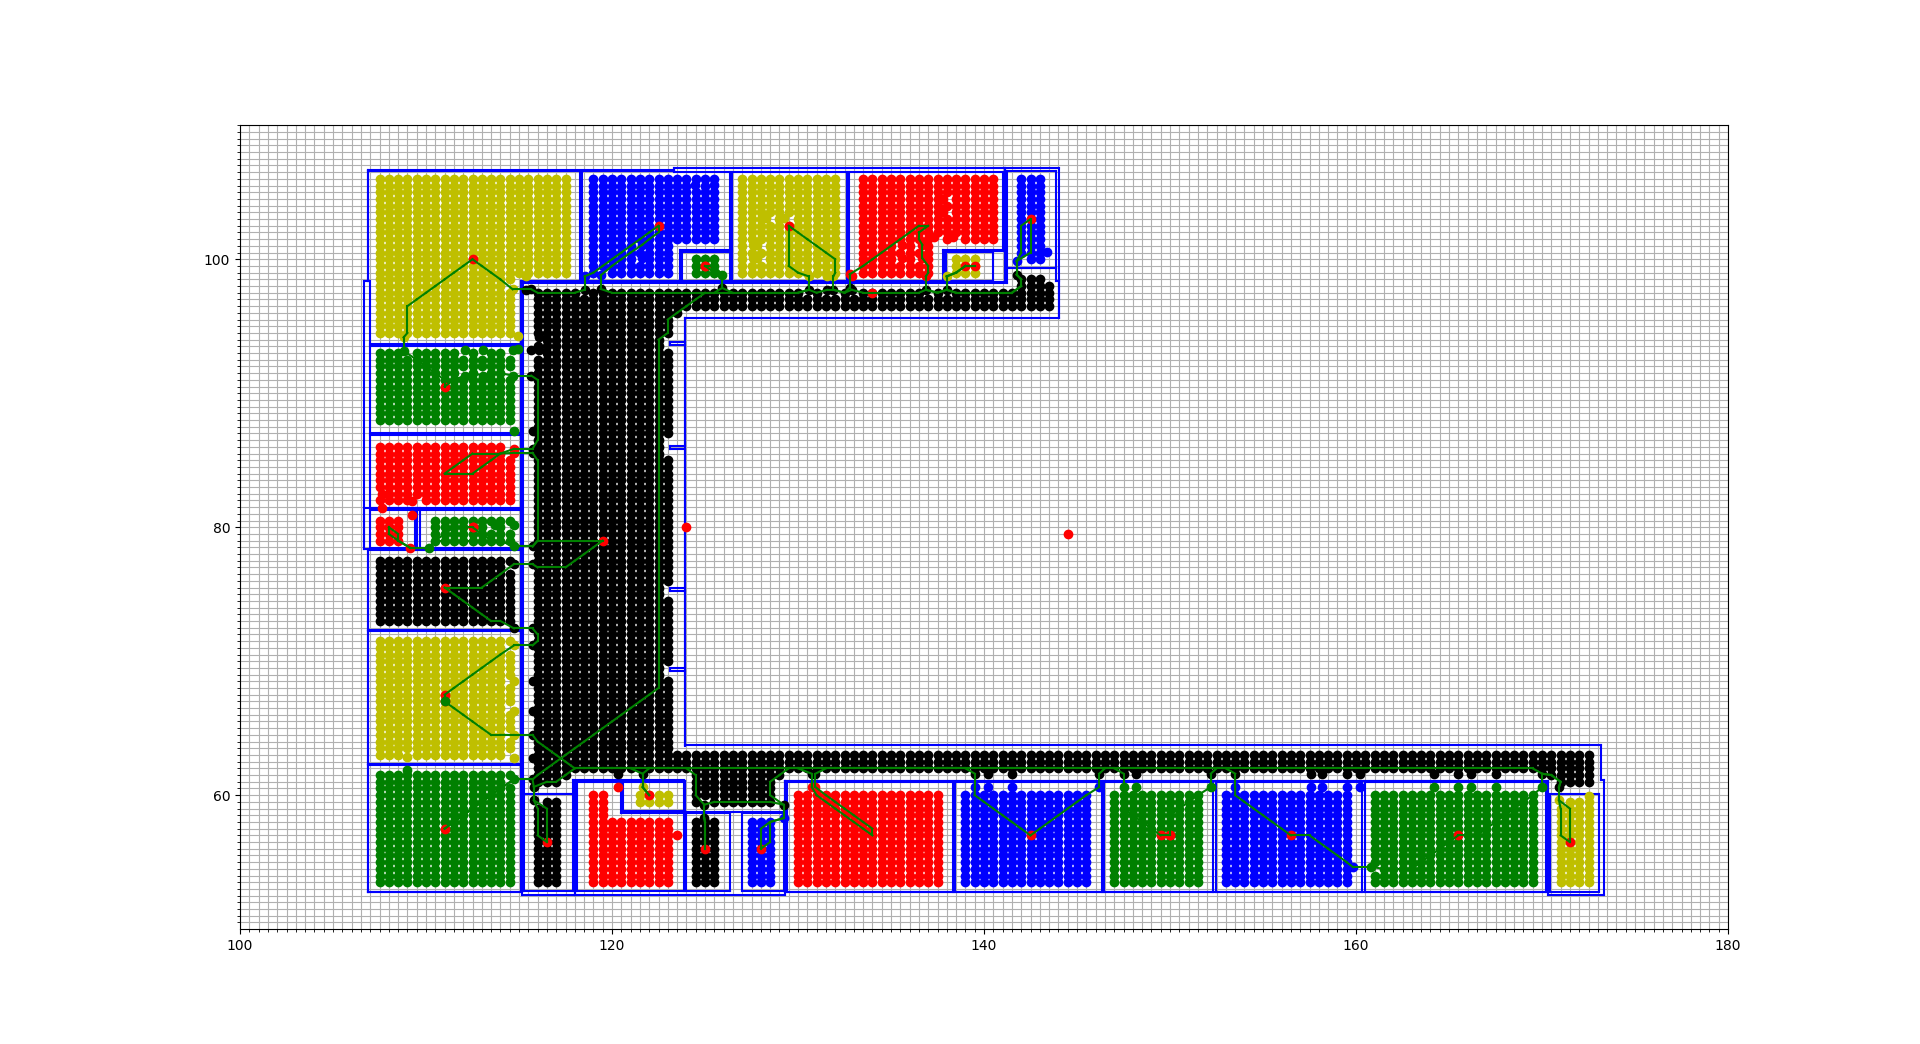
\includegraphics[width=1\textwidth]{fig/rum_labels.png}
    \label{}
    \caption[Design overview]{Rum knudepunkter}
\end{figure}


\begin{figure}[H]
    \centering
    \includegraphics[width=1\textwidth]{fig/hele_første_floorplan.png}
    \label{Rum knudepu}
    \caption[Design overview]{}
\end{figure}
\end{comment}


\section{RAC}
Comparing how the doors are plotted.
\begin{figure}[H]
    \centering
    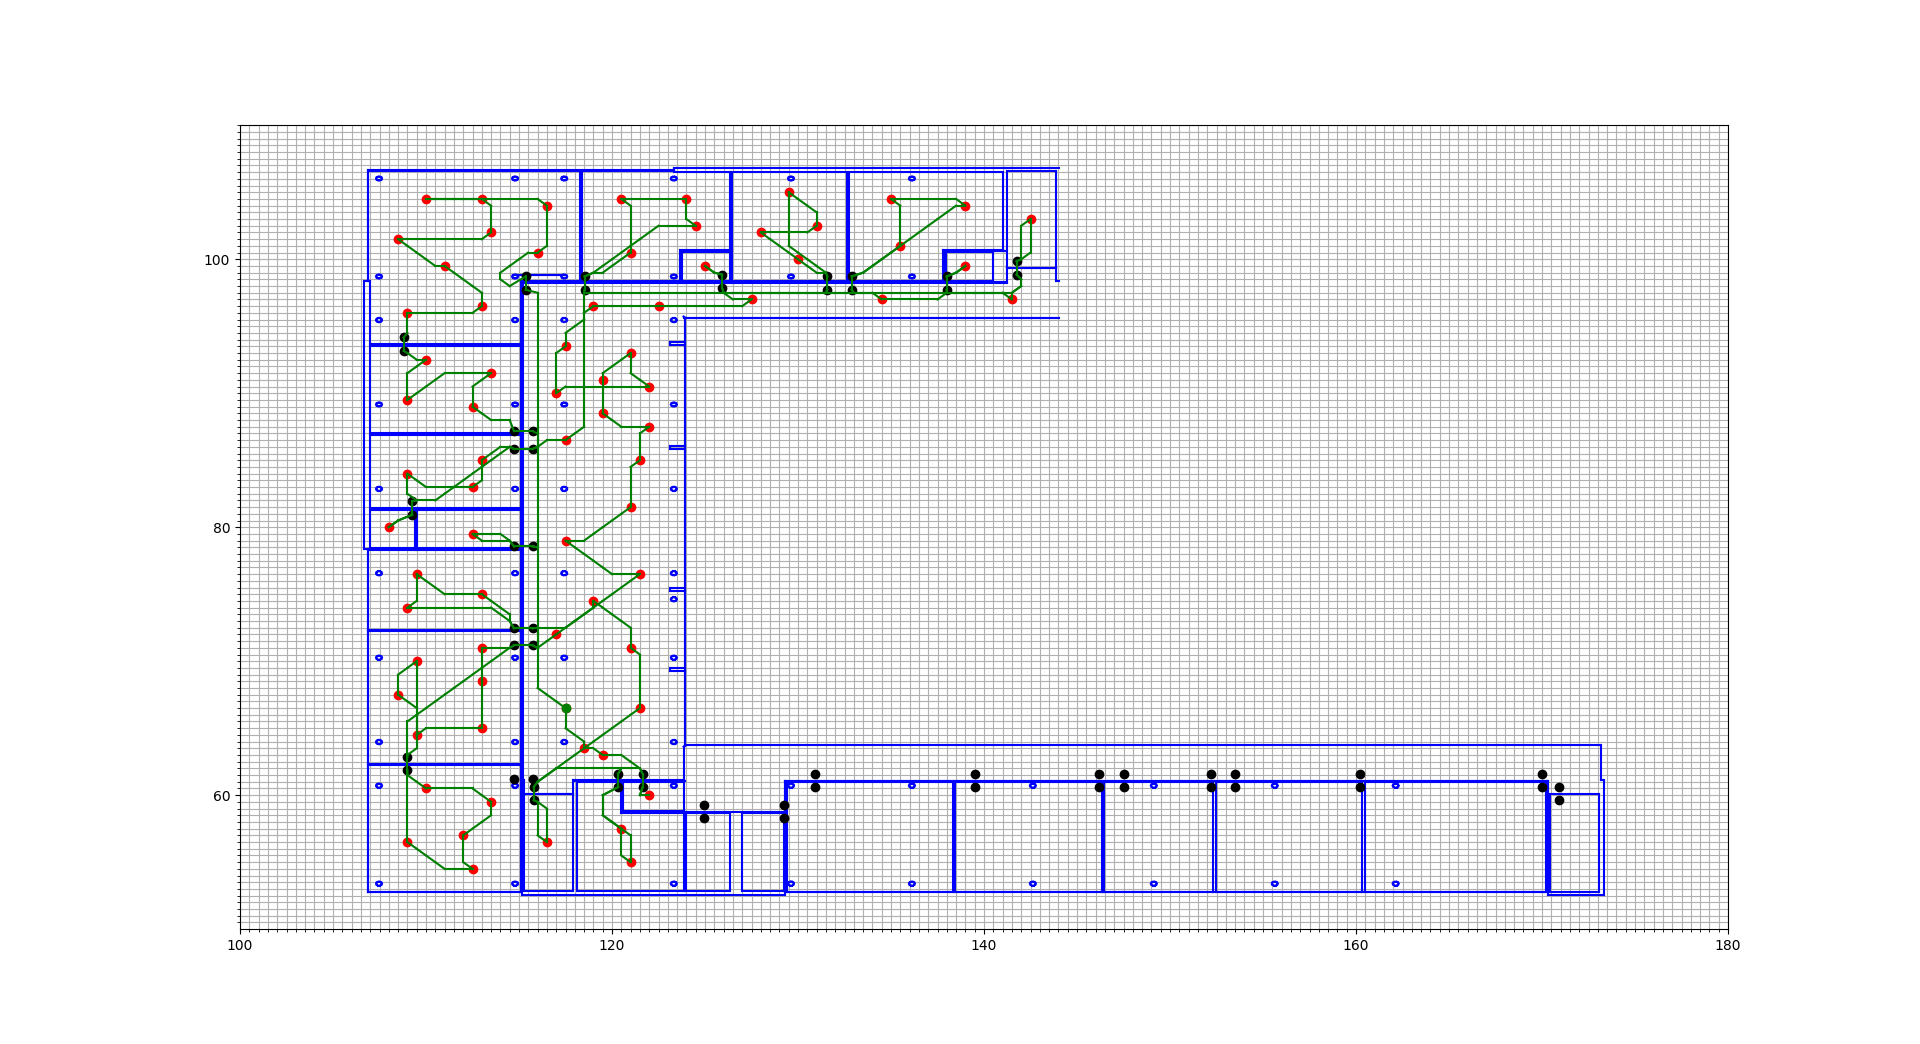
\includegraphics[width=1\textwidth]{fig/Resultater/Rac/-2.154_min_height_radius0.01.png}
    \label{Rum knudepu}
    \caption[Design overview]{}
\end{figure}


\begin{figure}[H]
    \centering
    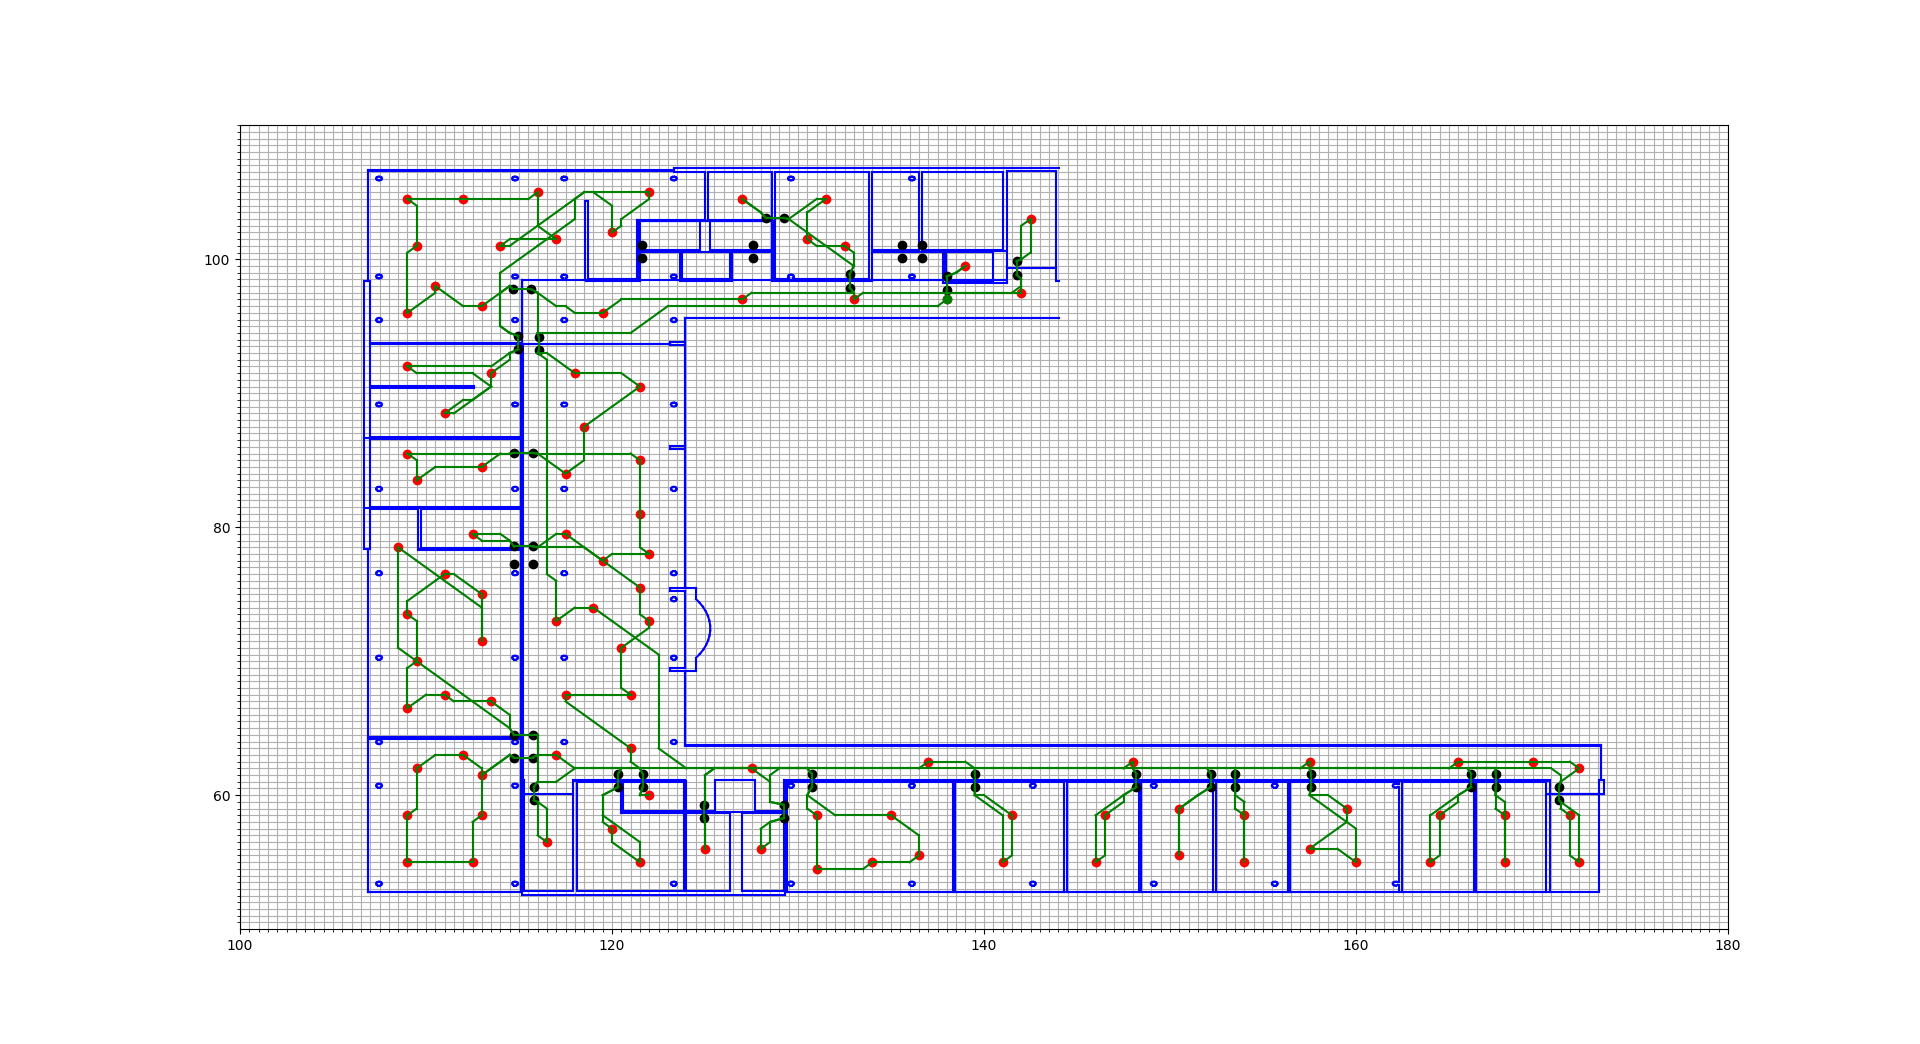
\includegraphics[width=1\textwidth]{fig/Resultater/Rac/-5.95_min_height_radius0.01.png}
    \label{Rum knudepu}
    \caption[Design overview]{}
\end{figure}


\begin{figure}[H]
    \centering
    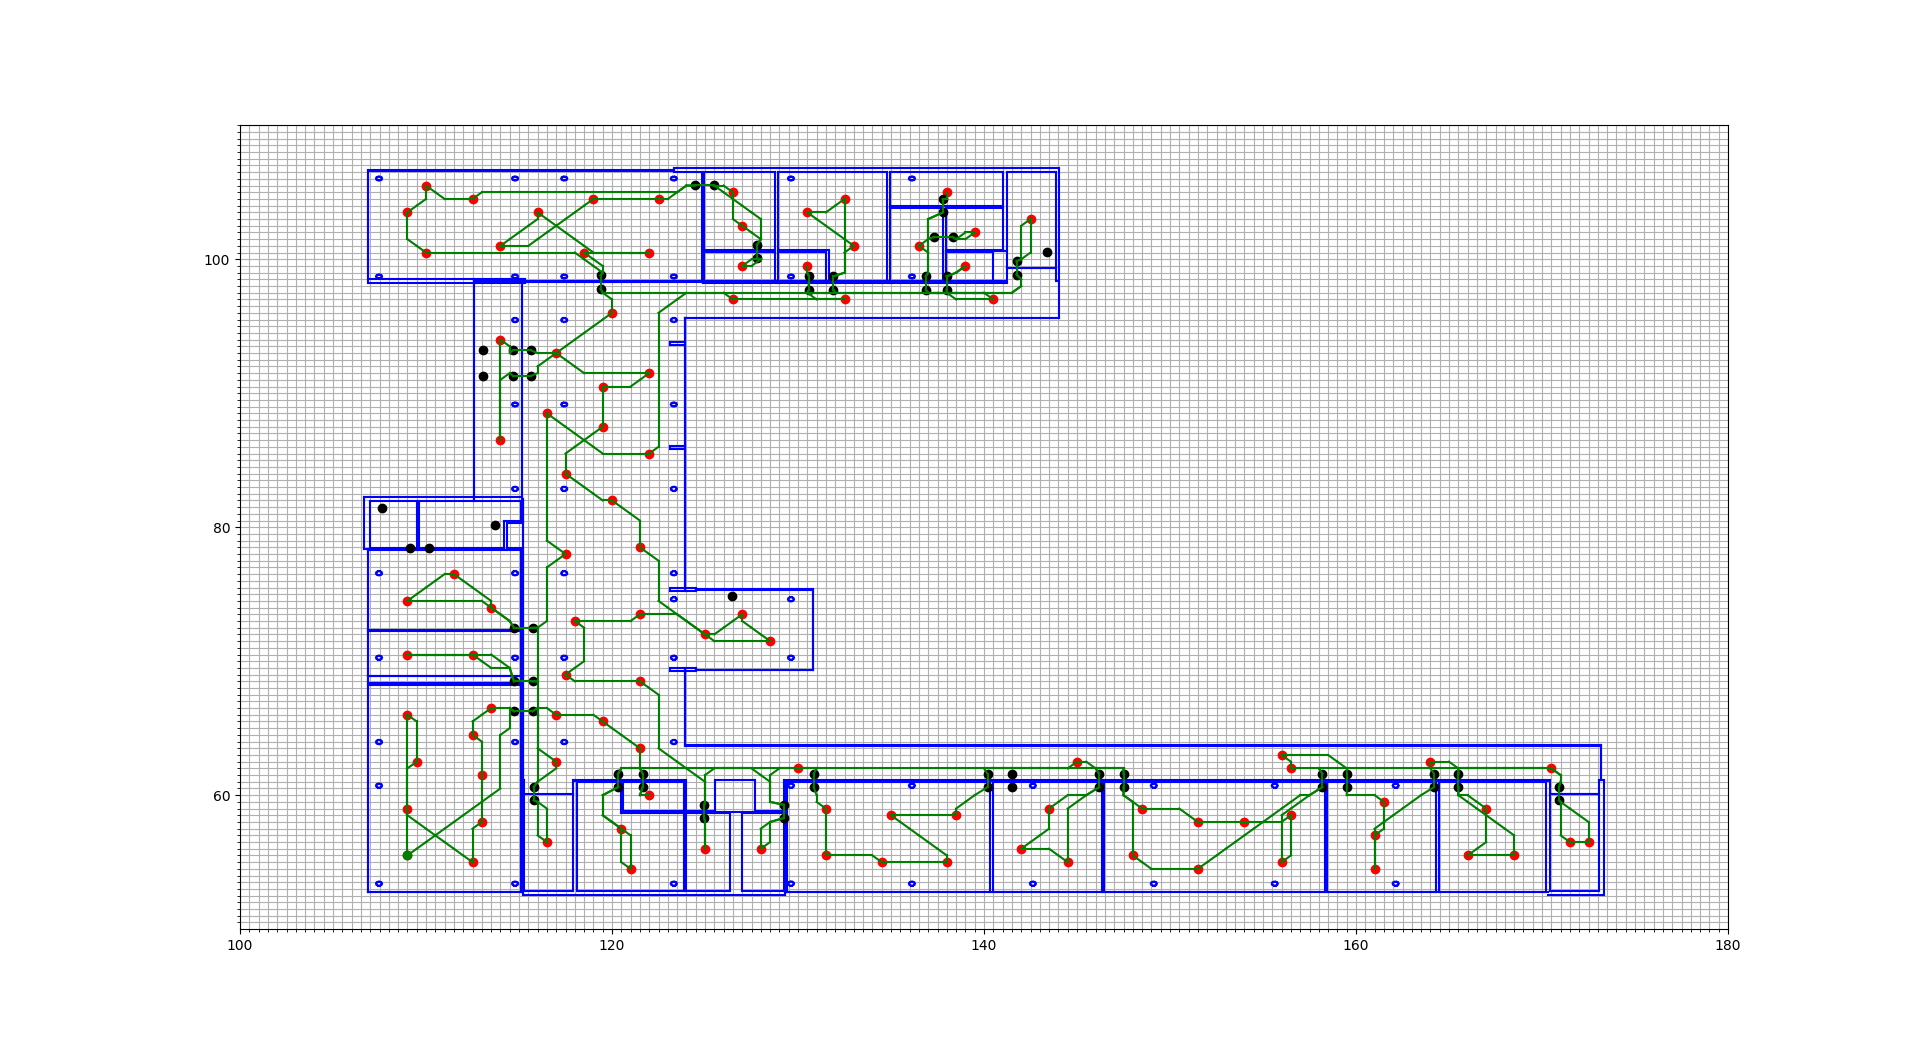
\includegraphics[width=1\textwidth]{fig/Resultater/Rac/-9.7_min_height_radius0.01.png}
    \label{Rum knudepu}
    \caption[Design overview]{}
\end{figure}


\section{Building 127}
- Checking 3 radius of different number of doors included.
How will the plotting work.
\begin{figure}[H]
    \centering
    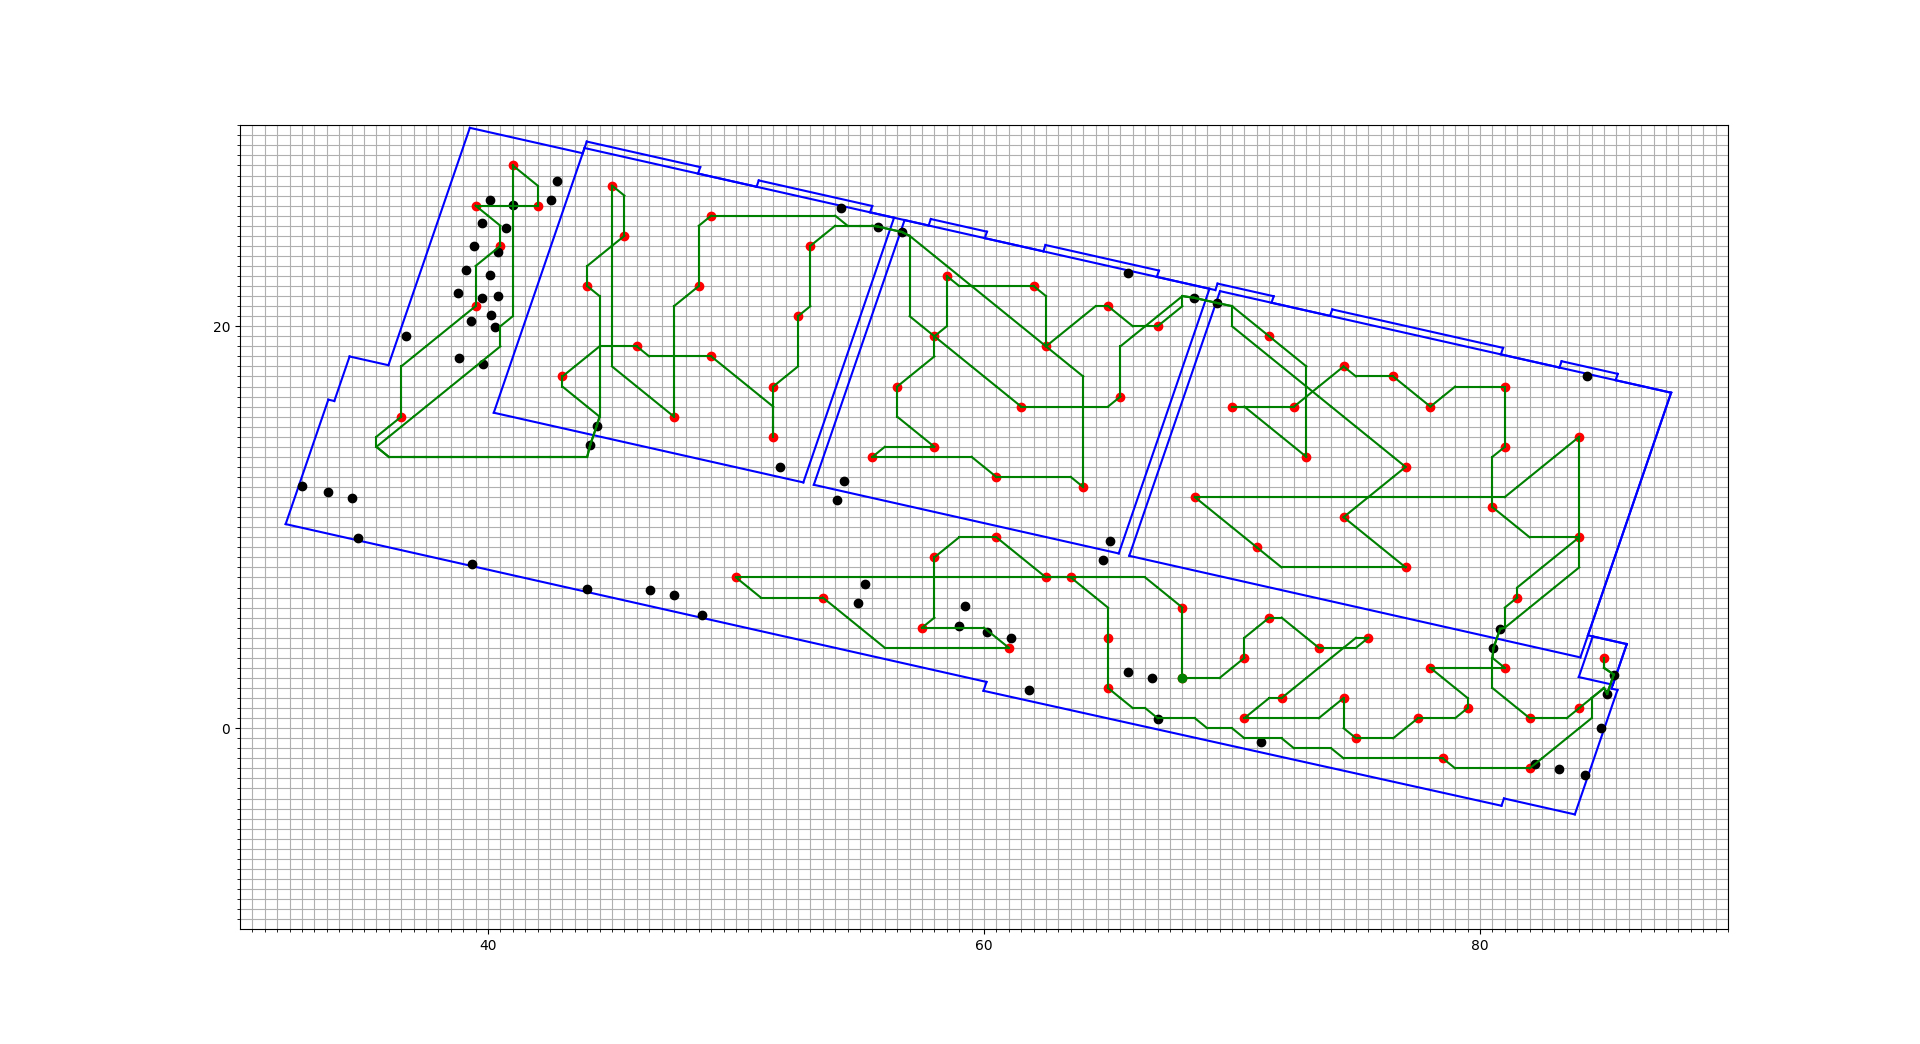
\includegraphics[width=1\textwidth]{fig/Resultater/127/0.31_min_height.png}
    \label{Rum knudepu}
    \caption[Design overview]{}
\end{figure}

\begin{figure}[H]
    \centering
    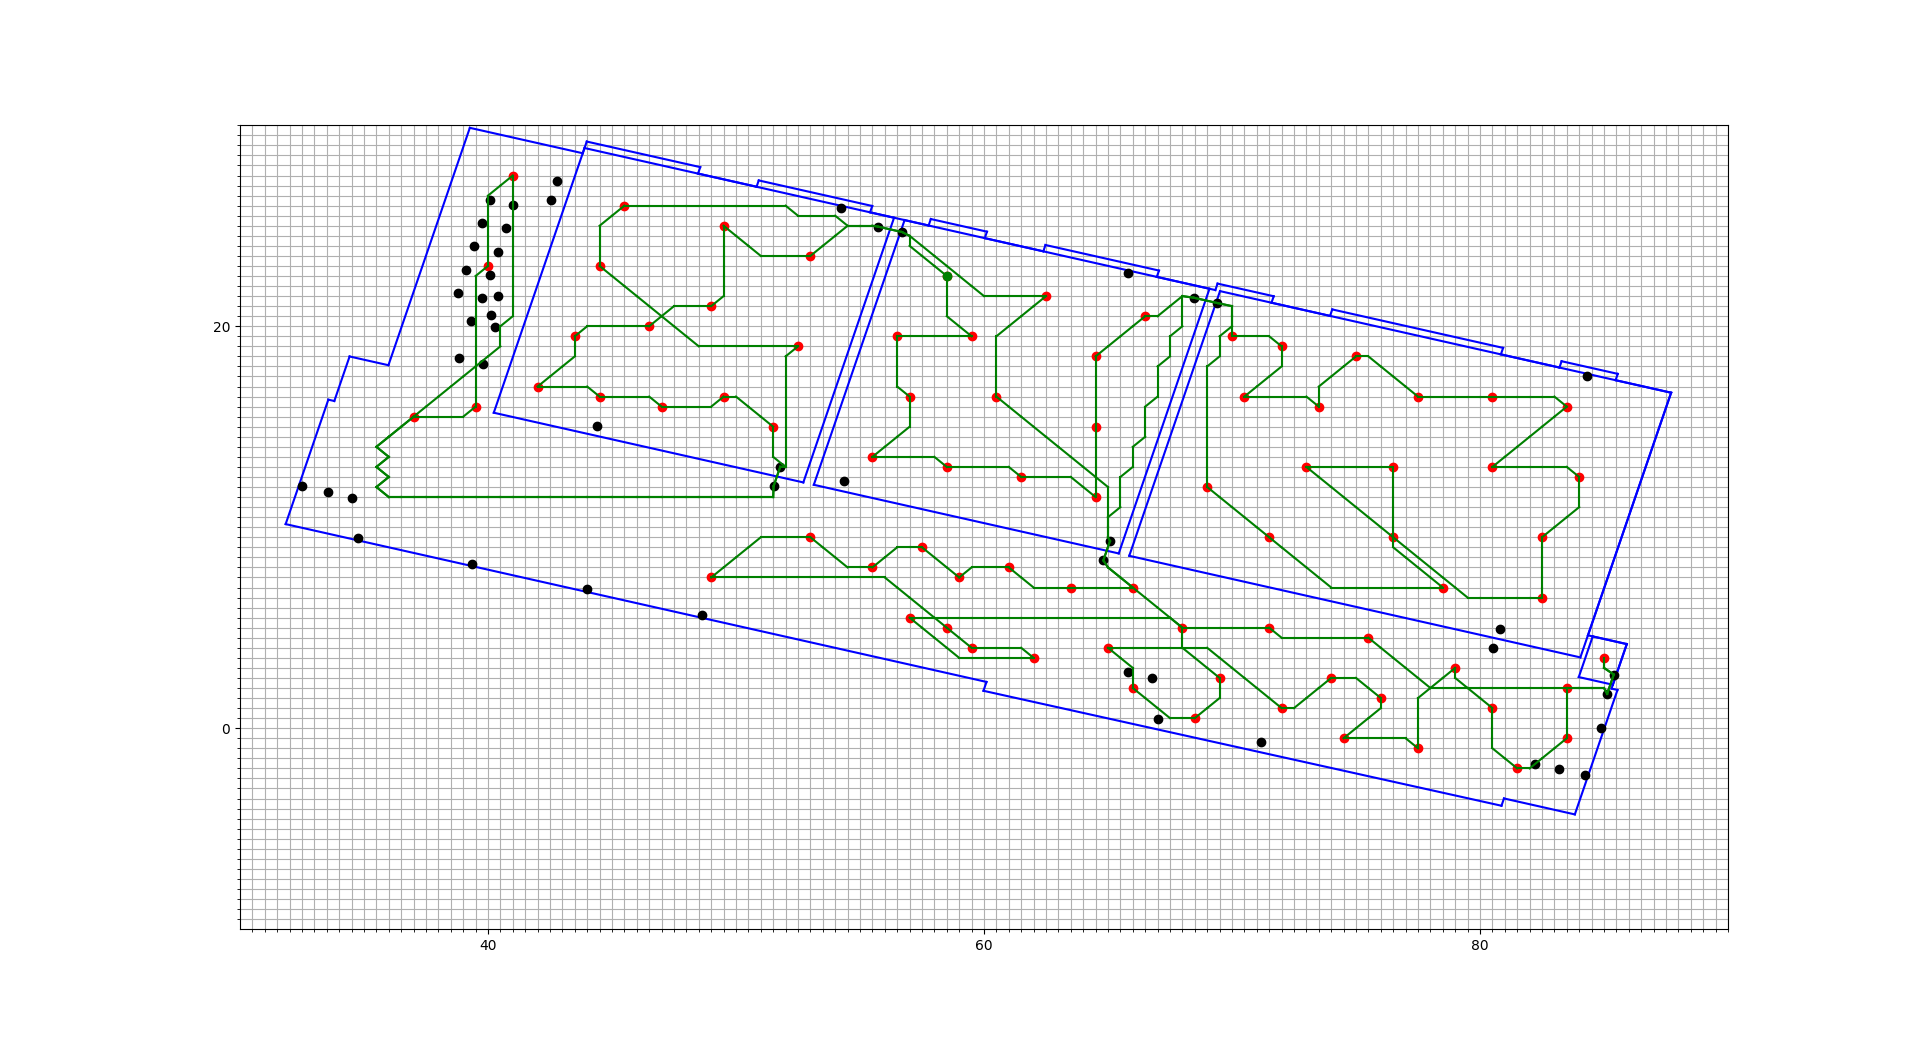
\includegraphics[width=1\textwidth]{fig/Resultater/127/0.31_min_height_radius0.1.png}
    \label{Rum knudepu}
    \caption[Design overview]{}
\end{figure}

\begin{figure}[H]
    \centering
    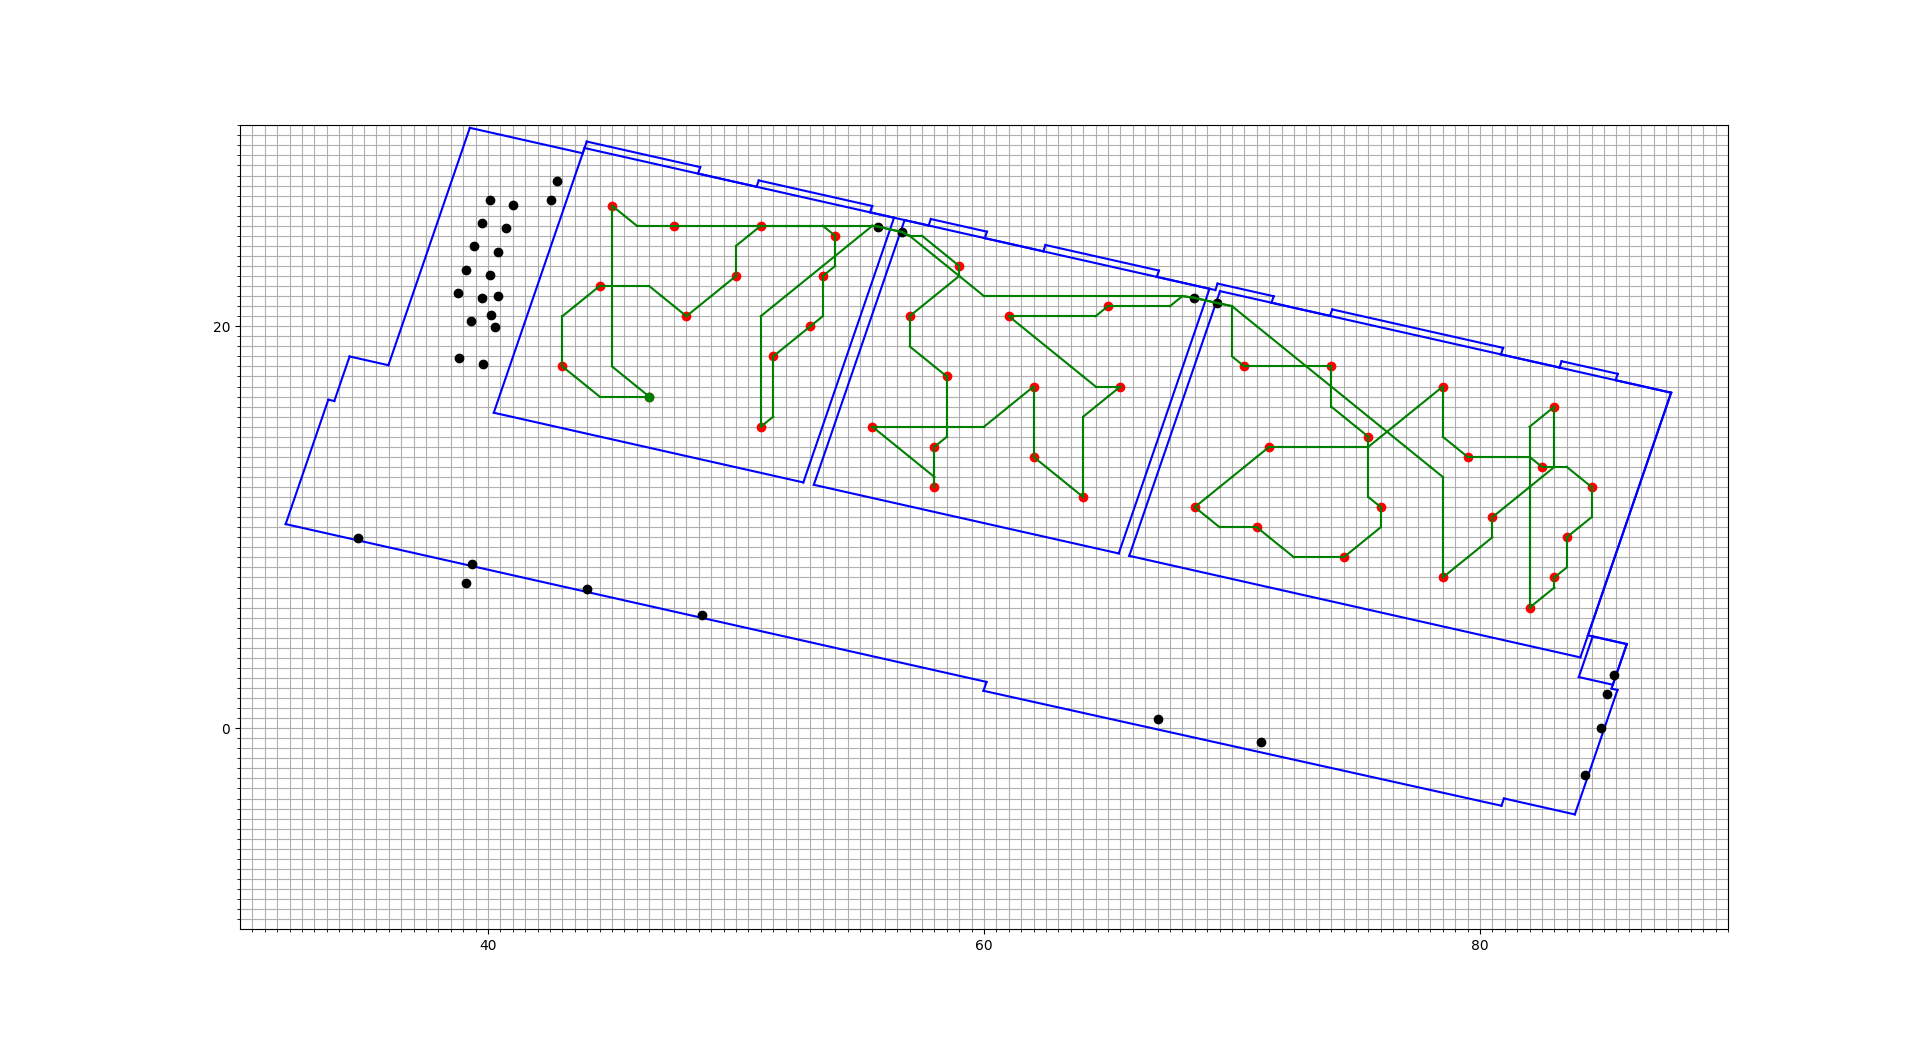
\includegraphics[width=1\textwidth]{fig/Resultater/127/0.31_min_height_radius0.01.png}
    \label{Rum knudepu}
    \caption[Design overview]{}
\end{figure}

on another floor
\begin{figure}[H]
    \centering
    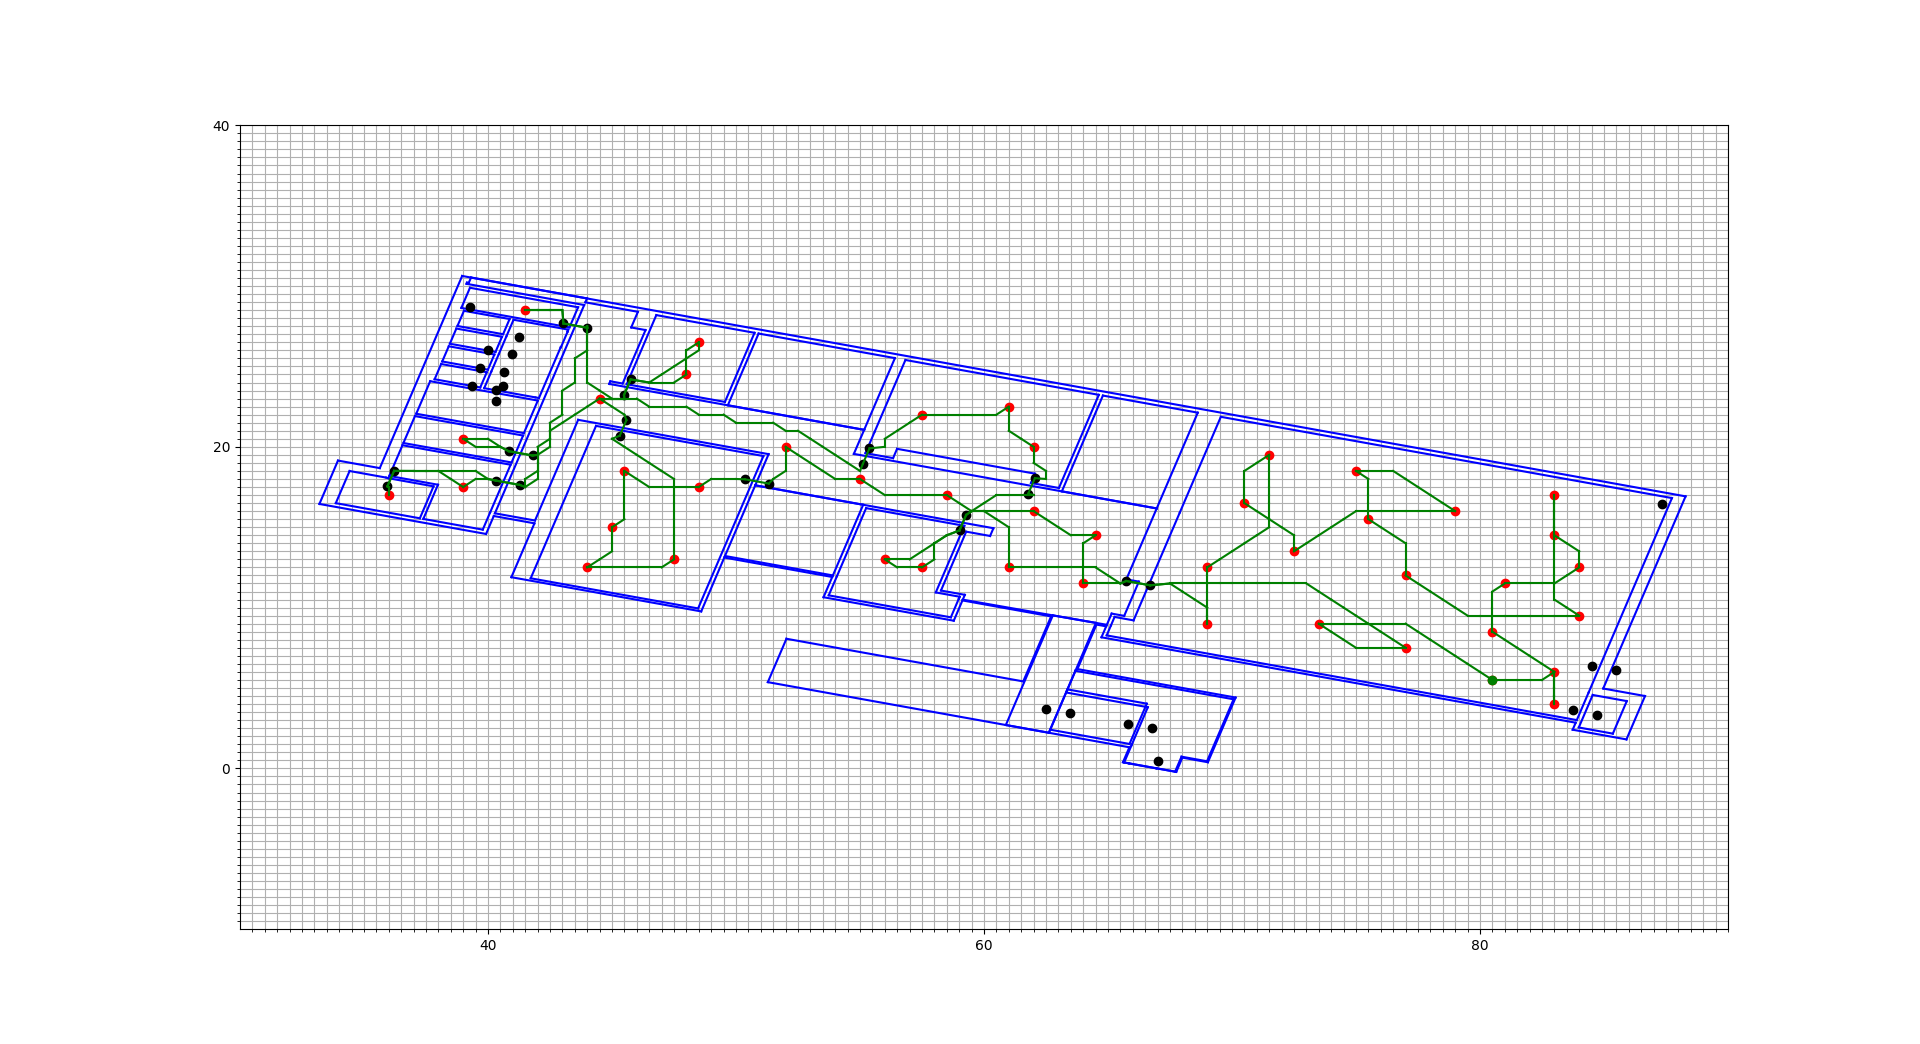
\includegraphics[width=1\textwidth]{fig/Resultater/127/5.36_min_height_radius1.png}
    \label{Rum knudepu}
    \caption[Design overview]{}
\end{figure}
\begin{figure}[H]
    \centering
    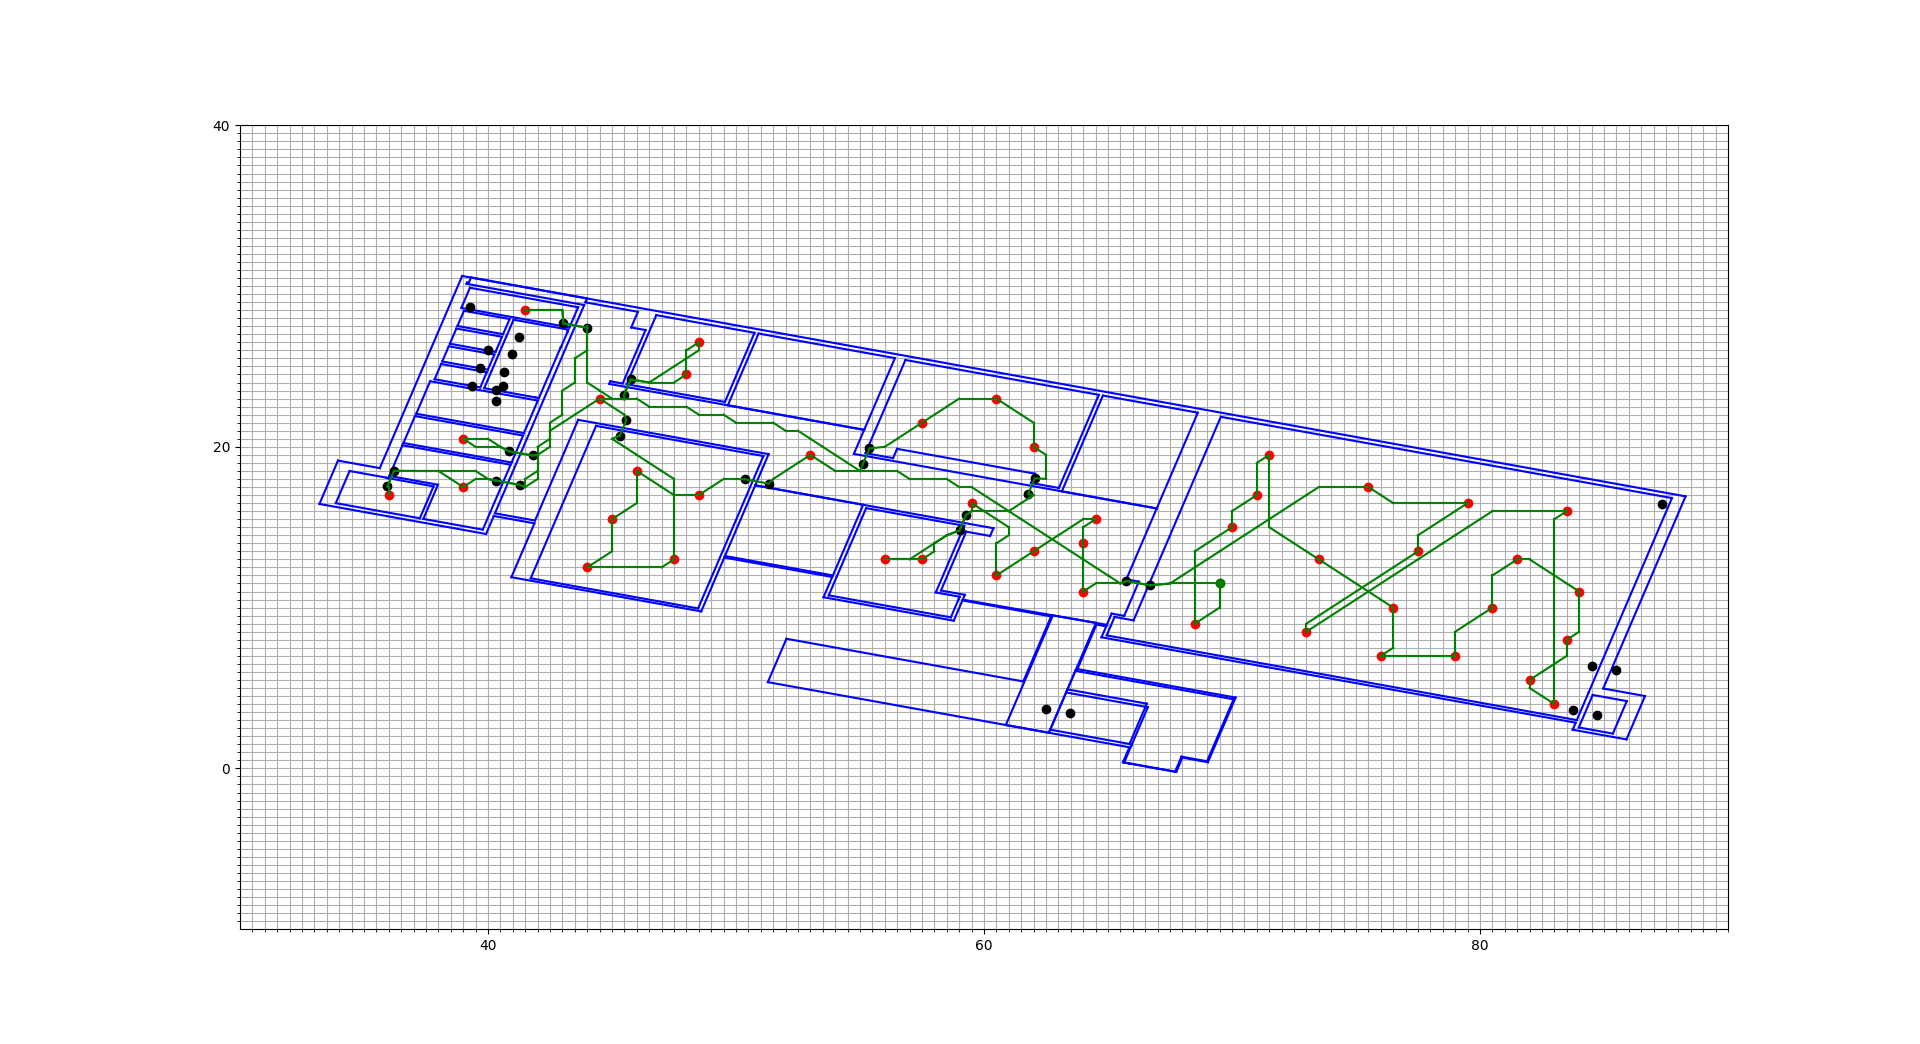
\includegraphics[width=1\textwidth]{fig/Resultater/127/5.36_min_height_radius0.1.png}
    \label{Rum knudepu}
    \caption[Design overview]{}
\end{figure}
\begin{figure}[H]
    \centering
    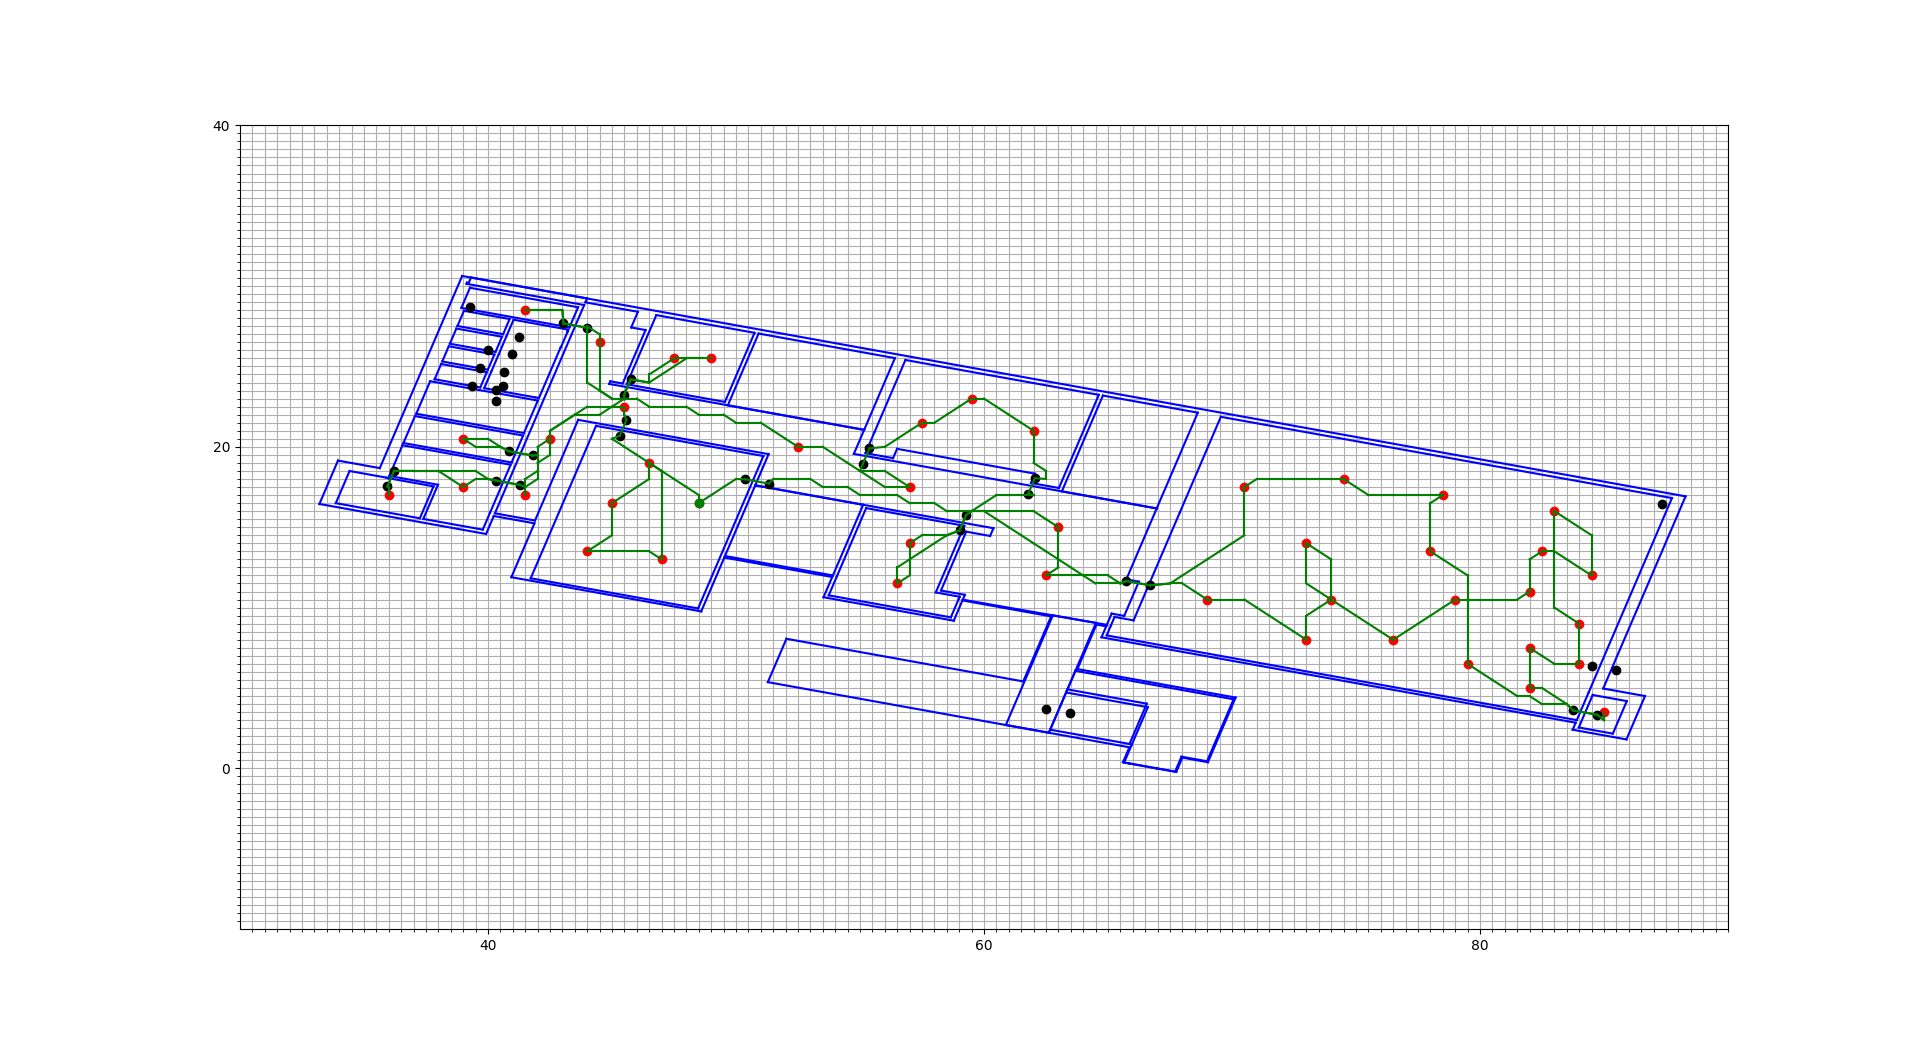
\includegraphics[width=1\textwidth]{fig/Resultater/127/5.36_min_height_radius0.01.png}
    \label{Rum knudepu}
    \caption[Design overview]{}
\end{figure}

Another floor again
Here there is not difference between using 0.01 radius or using 
\begin{figure}[H]
    \centering
    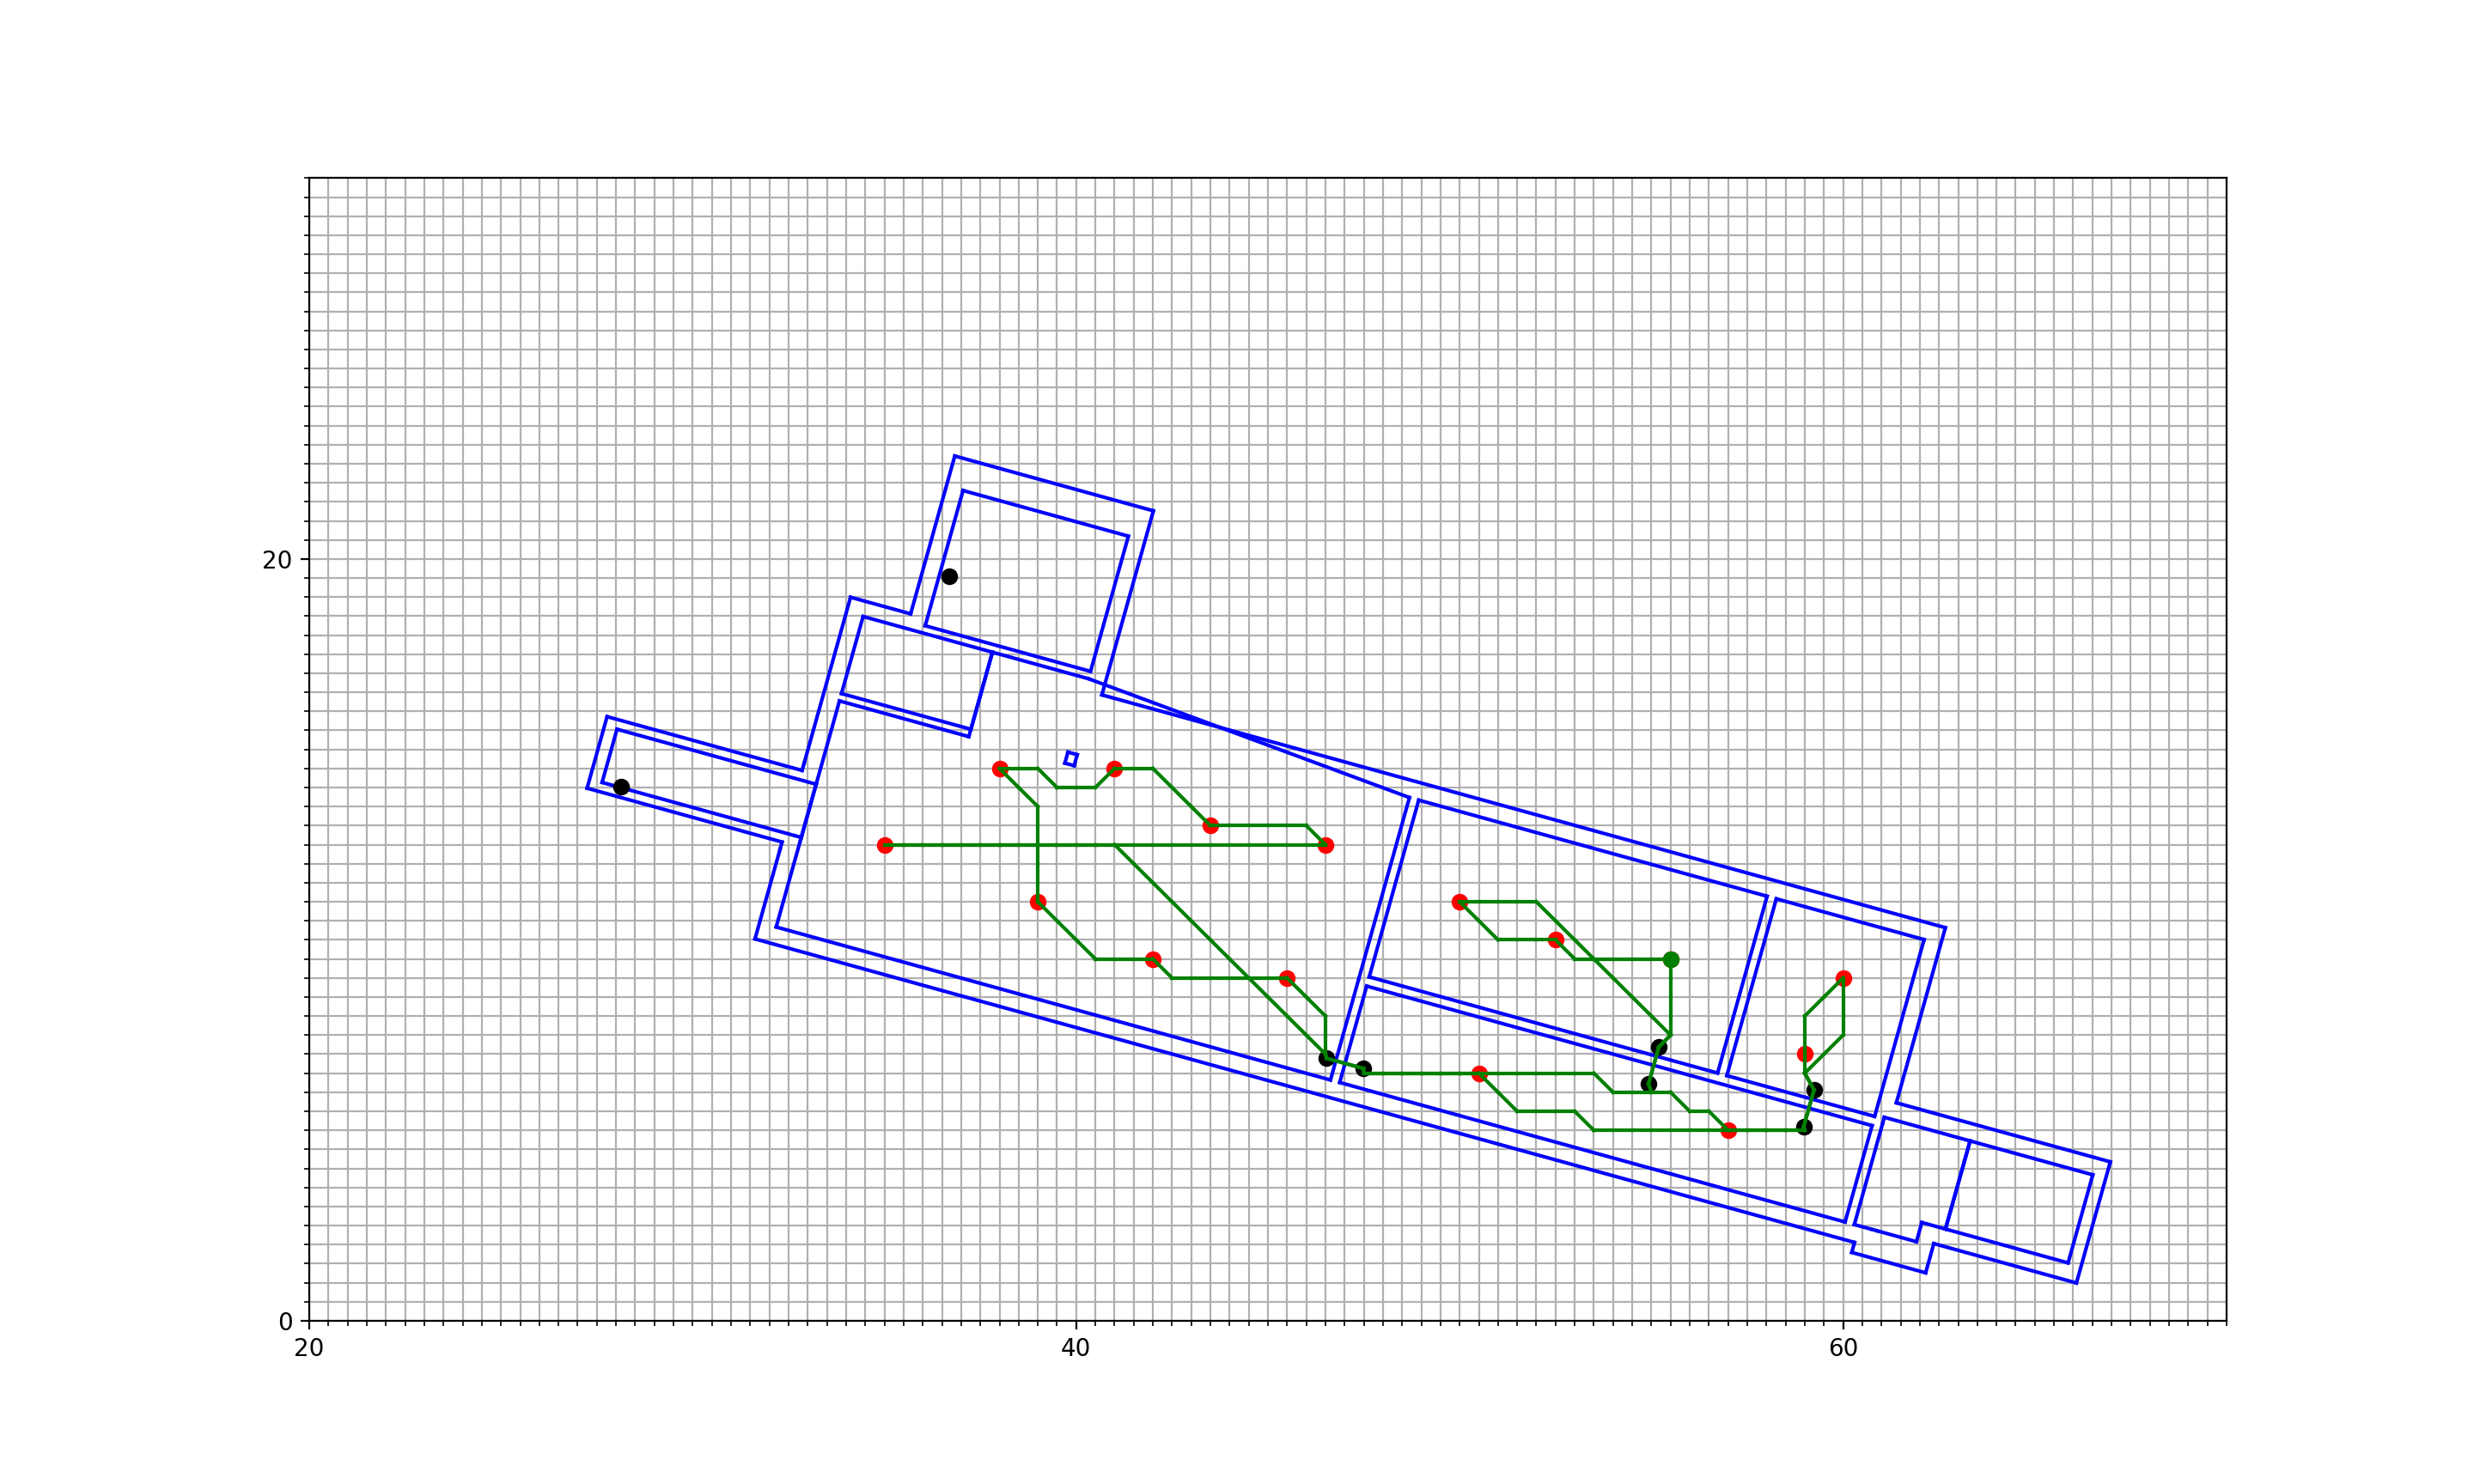
\includegraphics[width=1\textwidth]{fig/Resultater/127/-3.43_min_height.png}
    \label{Rum knudepu}
    \caption[Design overview]{}
\end{figure}